%
% Example of alignment models
%
%\begin{table}[t!]
%\begin{center}
%\begin{scriptsize}
%\begin{tabular}{l|p{60mm}}
%Passage	& Bob likes apples, which grow in his orchard.  He uses them for cider.  \\
%\hline
%Sequential & Bob likes apples, which grow in his orchard. $\rightarrow$ He uses them for cider. \\
%\hline
%RST & Bob likes apples, $\rightarrow$ which grow in his orchard. \\
% & Bob likes apples, which grow in his orchard. $\rightarrow$ He uses them for cider. \\
%
%
%\end{tabular}
%\end{scriptsize}
%%\vspace{-4mm}
%\caption{{\footnotesize \label{font-table} 
%An example of the alignments produced by the two discourse models.  While the sequential model aligns at sentence granularity capturing only intersentence information, the RST model aligns on finer EDU boundaries, capturing both inter/intrasentence alignments.
%}}
%\vspace{-4mm}
%
%\label{tab:examples}
%\end{center}
%\end{table}


\begin{figure}[t!]
\begin{center}
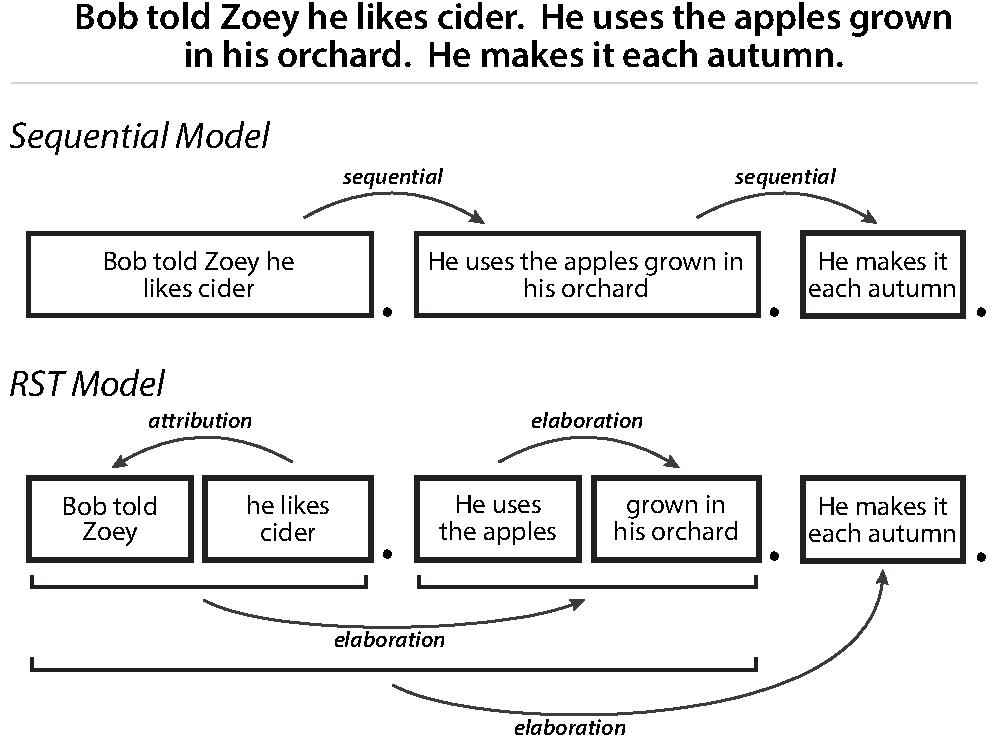
\includegraphics[width=75mm]{rst2a.pdf}
\vspace{-2mm}
\caption{{\small An example of the alignments produced by the two discourse models.  The sequential model aligns pairs of consecutive sentences, capturing intersentence associations such as \emph{cider--apples}, and \emph{orchard--autumn}.  The RST model generates alignment pairs from participants in all (binary) discourse relations, capturing both intrasentence and intersentence alignments, including 
\emph{apples--orchard, cider--apples}, and \emph{cider--autumn}.}}
% ms: I get the point, but there is value in brevity. Plus, maybe we should not use Bob as example :)
%the intersentence alignments above along with intrasentence and multi-sentence alignments, including \emph{Bob--cider, apples--orchard}, and \emph{cider--autumn}.}}
\vspace{-5mm}
\label{fig:examples}
\end{center}
\end{figure}

\vspace{-1mm}
\section{Approach}
\label{sec:approach}
\vspace{-1mm}

A written text is not simply a collection of sentences, but rather a flowing narrative where sentences and sentence elements depend on each other for meaning -- a concept known as cohesion~\cite{halliday2014cohesion}.  
%We make use of this to generate artificial alignment pairs using discourse.  
Here we examine two methods for generating alignment training data from free text that make use of cohesion: a shallow method that uses only intersentence structures, and a deep method that uses both intrasentence and intersentence structures.
We additionally attempt to separate the contribution of discourse from that of alignment in general by comparing these models against a baseline alignment model which aligns sentences at random.

The first model, the sequential discourse model (SEQ), considers that each sentence continues the narrative  of the previous one, and creates artificial question-answer pairs from all pairs of consecutive sentences.
% ms: no space
%This is similar to a right-attachment baseline in dependency parsing, 
%but operating at sentence granularity rather than word.
Thus, this model takes advantage of intersentence cohesion by aligning the content words\footnote{In pilot experiments, we found that aligning only nouns, verbs, adjectives, and adverbs yielded higher performance.} in each sentence with the content words in the following sentence.  For example, in the passage in Figure \ref{fig:examples}, this model would associate \emph{cider} in the first sentence with \emph{apples} and \emph{orchard} in the second sentence.

The second model uses RST to capture discourse cohesion both within and across sentence boundaries.  
We extracted RST discourse structures using an in-house parser~\cite{Surdeanu:15}, which follows the architecture introduced by Hernault et al.~\shortcite{hernault10} and Feng and Hirst~\shortcite{feng12}.
The parser first segments text into elementary discourse units (EDUs), which may be at sub-sentence granularity, then recursively connects neighboring units with binary discourse relations, such as \emph{Elaboration} or \emph{Contrast}.\footnote{The RST parser performs better on relations which occur more frequently.  We use only relations that occurred at least 1\% of the time.  This amounted to six relations: \emph{elaboration}, \emph{attribution}, \emph{background}, \emph{contrast}, \emph{same-unit}, and \emph{joint}. Using all relations slightly improves performance by 0.3\% P@1.} Our parser differs from previous work with respect to feature generation in that we implement all features that rely on syntax using solely dependency syntax. For example, a crucial feature used by the parser is the dominance relations of Soricut and Marcu~\shortcite{soricut2003}, which capture syntactic dominance between discourse units located in the same sentence. While originally these dominance relations were implemented using constituent syntax, we provide an equivalent implementation that relies on dependency syntax. The main advantage to this approach is speed: the resulting parser performs at least an order of magnitude faster than the parser of Feng and Hirst~\shortcite{feng12}. 

Importantly, we generate artificial alignment pairs from this imposed structure by aligning the governing text (nucleus) with its dependent text (satellite).\footnote{Pilot experiments showed that this direction of alignment performed better than aligning from satellite to nucleus.} 
 Turning again to the example in Figure \ref{fig:examples}, this RST-based model captures additional alignments that are both intrasentence, e.g., \emph{apples--orchard}, and intersentence, e.g., {\em cider--autumn}. 
% intersentence associations of the sequential baseline, in addition it finds an intrasentence association between \emph{apples} and \emph{orchard}. 

%\todo{The random alignment baseline (RND) was created in a similar fashion to the SEQ model, except that the sentences were randomly shuffled first.  In the open domain this shuffling took place within a document, and in the biology domain it was done across the entire of the textbook.}
